{\chapter{Physical Design}
\label{chap:PhysicalDesign}
In this chapter, we present the technical details of our implementation for the physical data structures that we will evaluate in our effort to answer a set of evaluation questions. This chapter comprises the following sections:


\begin{itemize}  
\item\textbf{Data Structures:}\\
In \ref{dataStructs}, we introduce the different data structures that we evaluate their performance in accordance to the evaluation questions. (\ref{dataStructs})
\item \textbf{Summary:}\\
Finally, we provide a summary for what we discussed in the chapter. (\ref{summary})
\end{itemize}
 
\section{Data Structures}
\label{dataStructs}

In the previous section, we presented the set of evaluation questions we aim to provide answers for. The questions are focusing on evaluating the performance of the data structures in different cases. In this section, we are providing a detailed explanation for the physical implementation of the data structures.

The data structures can be utilized by a graph database for storage and retrieval of graph data elements. We adopted the grouping of the data structures into two groups as presented by Paradies and Voigt in (\cite{Paradies2017}). 

The first group of data structures is the topology data structures. This group of data structures contains the data structures that can be used by graph databases for storing a directed graph topology.

The second group is for graph properties data structures. A properties data structure is designed to store the different properties that describe a vertex or an edge in the graph topology in a reach graph data model like RDF and PGM.

In (\ref{GraphTopolgyImp}), we are introducing our physical implementation details for data structures that belong to the group of graph topology data structures. Next, we are presenting our physical implementation details for data structures that belong to the group of graph properties data structures in (\ref{GraphPropertiesImp}).


\section{Graph Topology Structures}
\label{GraphTopolgyImp}

Graph topology data structures are designed exclusively to enable fast traversal across a graph. We are considering he logical representation of the graph topology data structures discussed in (\ref{chap:Background}) as our base for implementing their physical counterparts. 

In our physical implementation of the logical graph topology data structures, we have extended their definition for the stored graph from just a directed simple graph into a directed multi-graph. The multi-graph feature would mean that multiple edges can exist between the same two vertices. To distinguish multiple edges between the same two vertices, we store an edge label for each edge.

%\begin{figure}[th]
%\centering
%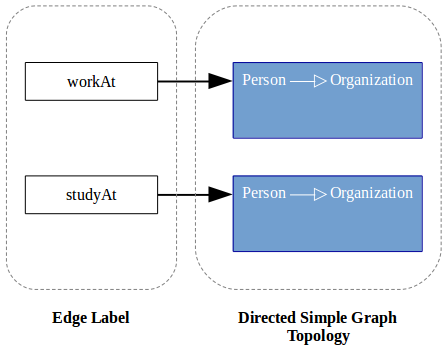
\includegraphics[width=5.5in]{Multi-graphTopology}
%\caption{Directed Multi-graph Topology}
%\label{fig_multiGraphTopology}
%\end{figure}

%In (\ref{fig_multiGraphTopology}), we are showing a block diagram for a logical representation of an example for a directed multi-graph. In the example, a directed multi-graph is stored between vertices of type \textit{"Person"} and \textit{"Organization"}, where the edges between the vertices are labeled as \textit{"workAt"} or \textit{"studyAt"}. We will store the directed multi-graph as a set of \textit{(key, value)} pairs, where the \textit{key} is the edge label and the \textit{value} is a graph topology data structure storing a directed simple graph for all edges labeled that have an edge label equal to \textit{key}.

We designed the graph topology data structures to facilitate the search, insert and retrieval of data in constant time by storing the data on multiple levels. Every data element we store in a graph topology data structure is consisted of three fields that represent a labeled relationship between two vertices. The three fields are \textbf{Source Vertex Id}, \textbf{Edge Label} and \textbf{Target Vertex Id}. An example for a three fields relationship is the relationship that exists in a social network graph between a post and its creator (e.g. \textit{post\_1 hasCreator person\_1}) with \textit{post\_1} represents the \textbf{Source Vertex Id}, \textit{hasCreator} represents the \textbf{Edge Label} and \textit{person\_1} represents the \textbf{Target Vertex Id}.

In the following subsections we are providing the technical details of our physical implementation for three graph topology data structures \textit{(Adjacency Matrix, Compressed Sparse Row and Adjacency List)}, as well as a parallel version of the \textit{Adjacency List} data structure that enables the ingestion of data from multiple parallel loaders. For every structure, we will present the building blocks we have utilized to build the data structure. Furthermore, we will explain the the mechanism and complexity for searching for an element inside the data structure.


%A graph is expressed mathematically as an ordered pair G = (E, V) with a set of edges E and a set of vertices V. In a directed graph, an edge (x, y) is a representation of the relationship between two vertices x and y, where x is the source vertex and y is the target vertex.



\begin{figure}
\centering
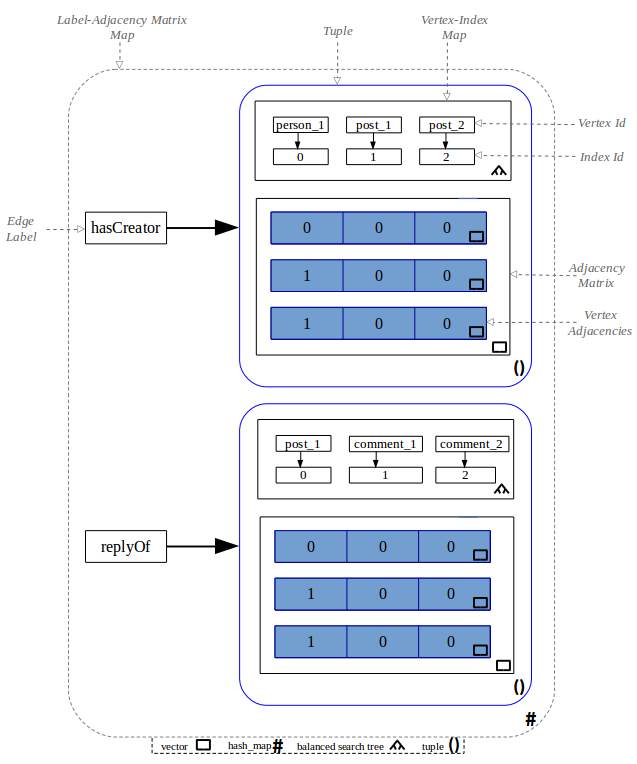
\includegraphics[height=7.8in]{adjacencyMatrix_physical}
\caption{Physical Representation of Labeled Adjacency Matrix}
\label{fig_adjacencyMatrix_physical}
\end{figure} 

\subsection{Adjacency Matrix}

In this subsection, we present our physical implementation of the labeled adjacency matrix data structure as one of the graph topology structures.

\begin{itemize}

\item{Structure:}

In (\ref{fig_adjacencyMatrix_physical}), we are presenting the underlying containers we utilized to implement the labeled adjacency matrix which which is basically defined as an adjacency matrix that is identified by the edge label of all possible edges between its vertices.

At the core of the structure, we store a two dimensional matrix serving as the \textit{Adjacency Matrix}. The size of the matrix is \textit{$n \times n$}. The row index id and column index id in the matrix are ranging from \textit{0} to \textit{n-1}. In addition, we store a \textit{Vertex-Index Map} that we use as a key/value store to associate each \textit{Vertex Id} with a corresponding \textit{Index Id} in the 2-d matrix. A \textit{Vertex Id} is always associated with one \textit{Index Id} which represents its row and column \textit{Index Id} in the 2-d matrix.

Each cell in the two dimensional matrix stores a boolean flag that indicates the existence of a relationship (i.e. flag = 1) between a source vertex which is associated with the row index of the cell, and a target vertex which is associated with the column index of the cell. A cell with "0" value means no relationship exists between the two vertices associated with the row and column index respectively.

%The \textit{Adjacency Matrix} space requirements is (\textit{O($n^2$)}) which for large graphs would be prohibitively expensive. For example, a graph of 10,000,000 vertex will require storage of size 11.6 petabyte.

In (\ref{fig_adjacencyMatrix_physical}), the \textit{Label-Adjacency Matrix Map} is a key/value store we use to associate every \textit{Edge Label} with a \textit{Tuple} that groups the \textit{Adjacency Matrix} and the \textit{Vertex-Index Map} in one container. Each \textit{Adjacency Matrix} will store the edge between the \textit{Source Vertex} and \textit{Target Vertex} which is labeled with the \textit{Edge Label} it's associated with.

\item{Insertion:}

To insert a new labeled relationship between two vertices into the structure, we first access the \textit{Label-Adjacency Matrix Map} using the \textit{Edge Label} as the access key. If no key exists with that \textit{Edge Label}, we insert a new key/value pair into the \textit{Label-Adjacency Matrix Map} with the key equal to the \textit{Edge Label} and the value is a \textit{Tuple} of empty \textit{Vertex-Index Map} and empty \textit{Adjacency Matrix}. Next, we retrieve the \textit{Index Ids} for the \textit{Source Vertex} and the \textit{Target Vertex} from the \textit{Vertex-Index Map}. In case any of the vertex ids of the source and target vertices not found in the \textit{Vertex-Index Map}, we insert a new key/value pair into the \textit{Vertex-Index Map} with the a key equal to the \textit{Source Vertex Id} and the value is \textit{m}, where \textit{m} is the number of pairs stored in the \textit{Vertex-Index Map} before the insertion. 

An insertion of new element(s) into the \textit{Vertex-Index Map} means that we must make a corresponding expansion in the \textit{Adjacency Matrix} to accommodate the relationship flags of the new elements(s). The \textit{Adjacency Matrix} is expanded by adding more columns and rows so that the final size of the matrix is equal to \textit{$m \times $m}, where \textit{m} is the number of pairs stored in the \textit{Vertex-Index Map}. The new cells added after expansion are all populated with a "0" value. 

Moreover, we use the \textit{Index Id} of the \textit{Source Vertex} as the row index and the \textit{Index Id} of the \textit{Target Vertex} as the column index in order to access a single cell at the \textit{Adjacency Matrix} and set the cell's flag to "1" to indicate an existence of a relationship between the \textit{Source Vertex} and the \textit{Target Vertex}.

\item{Searching:}

To search for a labeled relationship between two vertices in the structure, we first access the \textit{Label-Adjacency Matrix Map} using the \textit{Edge Label} as the access key. Next, we retrieve the \textit{Index Ids} for the \textit{Source Vertex} and the \textit{Target Vertex} from the \textit{Vertex-Index Map}. We use the retrieved \textit{Index Id} of the \textit{Source Vertex} as the row index and the \textit{Index Id} of the \textit{Target Vertex} as the column index in order to access a single cell at the \textit{Adjacency Matrix}.

If the cell holds a value of "1", it will mean that the relationship we are searching for does exist. A value of "0" would mean the opposite, that the relationship we are searching for does not exist.

The time complexity for the searching operation is the sum of complexity of three operations. First operation is accessing the \textit{Label-Adjacency Matrix Map} which has a complexity of \textit{O(1)}. Second operation is searching for the \textit{Index Id} for the \textit{Source Vertex} and the \textit{Target Vertex} from the \textit{Vertex-Index Map} which has a complexity of \textit{O(log(n) + log(n)) = O(2log(n))} where \textit{n} is the size of the \textit{Vertex-Index Map}. Third operation is accessing a cell in the \textit{Adjacency Matrix} which has a complexity of \textit{O(1)} for accessing the outer vector and \textit{O(1)} for accessing the inner vector which sums up to \textit{O(2)}.

By summing up the complexity of the three operations, the overall complexity of searching the structure is \textit{O(3 + 2log(n))}.

\item{Design Choices:}

We implemented the \textit{Label-Adjacency Matrix Map} as a static hash map to be the outer data container in the structure. The key of the hash map is the \textit{Edge Label}. As the number of \textit{Edge Labels} in a graph is not growing rapidly, the number of rehashing that is performed with the insertion of every new key will be limited. Meanwhile, the static hash map will give the best performance (\textit{O(1)}) for key look up operations on the \textit{Label-Adjacency Matrix Map}.

A graph can grow to include billions of vertices and hence the choice of a balanced search tree for implementing the \textit{Vertex-Index Map} as it guarantees a worst-case search or insert complexity for an element with \textit{O(log(size))}
(\cite{NSA}).

We chosen to implement the \textit{Adjacency Matrix} as a vector of vectors due to the the ability of the vector data structure to dynamically expand its capacity to store more elements in the run time. In addition, the vector data structure is storing its data contagiously in memory which enables the use of the principle of locality for efficient processing of the vector's data. Moreover, access operations on a vector is done in a constant time (\textit{O(1)}) which facilitates an efficient processing of the \textit{Adjacency Matrix's} data.

\end{itemize}

\subsection{Compressed Sparse Row (CSR)}

In this subsection, we present our physical implementation of the labeled compressed sparse row (CSR) data structure as one of the graph topology structures.



\begin{figure}[ht]
\centering
\hspace*{-0.4in}
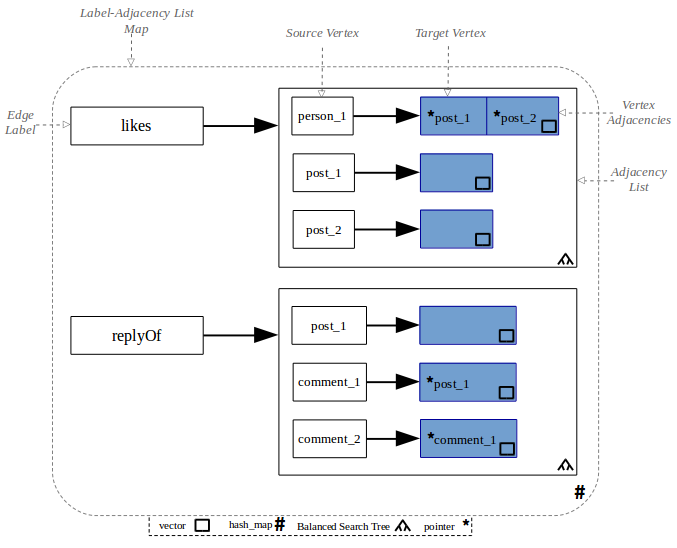
\includegraphics[width=6.8in]{adjacencyList_physical}
\caption{Physical Representation of Labeled Adjacency List}
\label{fig_adjacencyList_physical}
\end{figure}


\subsection{Adjacency List}
\label{adjList_physical}

In this subsection, we present our physical implementation of the labeled adjacency list data structure as one of the graph topology structures.

\begin{itemize}

\item{Structure:}

In (\ref{fig_adjacencyList_physical}), we are presenting the underlying containers we utilized to implement the labeled adjacency list which is basically defined as an adjacency list that is identified by the edge label of all possible edges between its vertices.

At the core of the structure, we store the \textit{Adjacency List} as a key/value store to associate each \textit{Source Vertex} with a corresponding sorted list of \textit{Target Vertices}. Each element of the list of \textit{Target Vertices}, is a direct pointer towards the key/value pair of the referenced \textit{Target Vertex} in the \textit{Adjacency List}.

In (\ref{fig_adjacencyList_physical}), the \textit{Label-Adjacency List Map} is a key/value store we use to associate every \textit{Edge Label} with an \textit{Adjacency List}. Each \textit{Adjacency List} will store the edge between the \textit{Source Vertex} and \textit{Target Vertex} which is labeled with the \textit{Edge Label} it's associated with.

\item{Insertion:}

To insert a new labeled relationship between two vertices into the structure, we first access the \textit{Label-Adjacency List Map} using the \textit{Edge Label} as the access key. If no key exists with that \textit{Edge Label}, we insert a new key/value pair into the \textit{Label-Adjacency List Map} with the key equal to the \textit{Edge Label} and the value is an empty \textit{Adjacency List}. Next, we access the \textit{Adjacency List} using the \textit{Source Vertex} as the key. Additionally, we retrieve a pointer to the key/value pair entry of the \textit{Target Vertex} from the \textit{Adjacency List}. In case we didn't find an entry with the given \textit{Source Vertex} or \textit{Target Vertex}, we insert a new key/value pair into the \textit{Adjacency List} with the key equal to the \textit{Vertex Id} and the value is an empty list. Lastly, we insert the pointer of the \textit{Target Vertex} into the list of \textit{Target Vertices} of the \textit{Source Vertex}, ensuring the insertion leaves the list sorted by the \textit{Vertex Id}.

\item{Searching:}

To search for a labeled relationship between two vertices in the structure, we first access the \textit{Label-Adjacency List Map} using the \textit{Edge Label} as the access key. Next, we access the \textit{Adjacency List} using the \textit{Source Vertex} as the key. Lastly, we search the list of \textit{Target Vertices} for a pointer to the given \textit{Target Vertex}.

The time complexity for the searching operation is the sum of complexity of three operations. First operation is accessing the \textit{Label-Adjacency List Map} which has a complexity of \textit{O(1)}. Second operation is is accessing the \textit{Adjacency List} which has a complexity of \textit{O(log(n))}, where \textit{n} is the number of key/value pairs stored in the \textit{Adjacency List}. Third operation is searching the list of \textit{Target Vertices} for a pointer to the given \textit{Target Vertex} which has a complexity of \textit{O(m)}, where \textit{m} is the size of the \textit{Target Vertices} list.

By summing up the complexity of the three operations, the overall complexity of searching the structure is \textit{O(1 + log(n) + m)}.

\item{Design Choices:}

Similar to the \textit{Label-Adjacency Matrix Map}, we implemented the \textit{Label-Adjacency List Map} as a static hash map to be the outer data container in the structure. The key of the hash map is the \textit{Edge Label}. The static hash map will give the best performance (\textit{O(1)}) for key look up operations on the \textit{Label-Adjacency List Map}.

A graph can grow to include billions of vertices and hence the choice of a balanced search tree for implementing the \textit{Adjacency List} as it guarantees a worst-case search or insert complexity for an element with \textit{O(log(size))}
(\cite{NSA}).

We chosen to implement the list of \textit{Target Vertices} as a vector due to the the ability of the vector data structure to dynamically expand its capacity to store more elements in the run time. In addition, the vector data structure is storing its data contagiously in memory which enables the use of the principle of locality for efficient processing of the vector's data. Moreover, access operations on a vector is done in a constant time (\textit{O(1)}) which facilitates an efficient processing of the list elements. Keeping the list of \textit{Target Vertices} sorted, makes the search for specific element in the list more efficient by utilizing a range of searching algorithms (e.g. binary search).

\end{itemize}


\subsection{Parallel Adjacency List}

In this subsection, we present our physical implementation of a parallel version of the adjacency list data structure. The parallel adjacency list differs from the adjacency list presented in (\ref{adjList_physical}) in that the parallel adjacency list enables the ingestion of data from multiple parallel loaders simultaneously.



\section{Graph Properties Structures}
\label{GraphPropertiesImp}


\subsection{Universal Table}


\subsection{Emerging Schema}


\subsection{Schema Hashed Map}


\subsection{Parallel Schema Hashed Map}


\section{Summary}
\label{summary}

}